\documentclass{article}
\usepackage[utf8]{inputenc}
\usepackage[T1]{fontenc}
\usepackage{lmodern}
\usepackage{amsmath, amssymb}
\usepackage{graphicx}
\usepackage{float} 
\usepackage{hyperref}
\usepackage{subcaption}
\usepackage{geometry}
\usepackage{bookmark}
\geometry{margin=1in}
\usepackage{pgfplots}
\pgfplotsset{compat=1.17}


\title{Comparing Machine Learning and Deep Learning Models with Attention Mechanisms for Multiple Authorship Attribution}
\author{Richard Čerňanský, Ing. Juraj Petrík}
\date{\today}

\begin{document}
\maketitle

\begin{abstract}
    Authorship attribution (AA) in source code is crucial for plagiarism detection, 
    forensic analysis, and software maintenance, especially when author 
    information is missing or ambiguous. This field is not as well explored 
    as the written communication AA and there are new models to be tested 
    on different sized dataset. This study compares traditional 
    machine learning models, such as Random Forests trained on TF-IDF 
    tokenized representations, with deep learning models, including BERT 
    and an Attention-based Neural Network (AttentionNN), for the task of 
    multiple authorship attribution. We evaluate different representations 
    of source code, including raw tokenized text and Abstract Syntax Tree (AST) 
    structures, to determine their effectiveness in distinguishing authorship. 
    The models are tested on a dataset of 3,004 C language functions from 
    Google Code Jam spanning 2009–2018, assessing their accuracy, precision, 
    recall, and training efficiency across varying author set sizes. 
    Our findings highlight the strengths and limitations of each approach, 
    showing that while deep learning models, particularly BERT trained on 
    raw source code, achieve the highest accuracy, Random Forests offer 
    competitive results with significantly lower computational cost. 
    The study also explores the impact of function complexity on model 
    performance, revealing that AttentionNN benefits from structural 
    complexity while struggling with short functions. The results emphasize 
    the trade-offs between accuracy, computational efficiency, and data 
    representation, providing insights into the optimal model selection 
    for source code authorship attribution.   
\end{abstract}

\section{Introduction}

Authorship attribution in source code analysis is a crucial task 
with applications in plagiarism detection, forensic investigations, and 
intellectual property protection, but also software maintenance
and software quality analysis, where the information about an author 
is missing, inaccurate or ambiguous.
Given a function written in a programming
language, determining its author requires capturing distinct stylistic 
patterns. Traditional machine learning (ML) methods, such as Random 
Forests trained on TF-IDF tokenized representations, have shown promise 
in text-based authorship identification. However, recent advancements 
in deep learning (DL) have introduced transformer-based models, such as 
BERT, which leverage contextual embeddings and self-attention mechanisms 
to extract more meaningful patterns from textual data.

Despite the success of deep learning models in natural language 
processing (NLP), their application to source code authorship attribution on different dataset sizes. 
remains relatively unexplored. Unlike natural language, source code 
exhibits a more rigid syntax and structure, making its representation 
a key challenge. Several approaches have been proposed, ranging from 
direct tokenized representations of the raw source code to abstract 
syntax tree (AST) transformations that capture program logic. However, 
it remains unclear which type of representation is most effective for 
distinguishing authorship across different levels of dataset complexity.

This study systematically compares machine learning and deep learning 
models, including Random Forests, BERT trained on tokenized source code, 
BERT trained on AST representations, and an Attention-based Neural Network 
(AttentionNN) utilizing AST-derived node-to-node paths. The evaluation is 
conducted on a dataset of 3,004 C language functions from Google Code Jam 
(GCJ) spanning 2009 to 2018 \cite{gcj}. The models are assessed based on their 
accuracy, precision, recall, and training efficiency across different 
author set sizes.

Through this comparison, we aim to determine which model best balances 
accuracy and computational efficiency, as well as the effectiveness of 
different function representations for authorship attribution.

\section{Methods}

\subsection{Source code representation}

In the paper \cite{information}, authors present division of features based on the method they use for extraction: 
    
\begin{itemize}

    \item \textbf{Stylometric features:} 
    They express the structural characters that represent the author’s preference for different statements, keywords, nesting sizes, etc.
    \item \textbf{N-gram features:}
    N-gram is a contiguous sequence of an n byte, character, or words extracted from the source. A sliding that has a fixed length generates 
    the sequence.
    \item \textbf{Graph based features:}
    These capture underlying traits in the code such as deeply nesting code, control flow and data flow.
    It includes : AST, Program Dependency Graph (PDG), Control Flow Graph (CFG), RFG.
    \item \textbf{Behavioral features:}
    This type completely different from the previous as it is not looking at the source code itself
    but rather on the way that the program of the source code communicates with the computer.
    In this category there are dynamic features which collect runtime measurements as CPU and memory usage.
    Instruction features that are retrieved from binaries and reflect code properties like registers or immediate operands.
    \item \textbf{Neural Networks Generated Representations of Source Code or Features:}
    Lastly, in recent years, neural networks have been increasingly utilized 
    to generate representations (such as embeddings) of source code. This 
    approach is also applied in this thesis, using AST analysis to provide 
    input for the neural network.

\end{itemize}

\subsection{Abstract Syntax Tree}

\quad Based on the full definition \cite{sun2023AST} Abstract syntax tree (AST) is a tree-based representation of source code, where nodes represent various elements of the source code 
and paths represent relationships of the structure. AST is an inseparable part of compilation process for many reasons. It is used as an 
intermediate representation of program utilized for optimization and generation of machine code. Nodes of the tree can be either internal 
(non-leaf) or leafs. Internal nodes define the program's constructs or operations for their children. Leaf nodes store the actual textual value. 


Below is an example of a simple C function and its corresponding Abstract Syntax Tree (AST):
\begin{verbatim}
int add(int a, int b) {
    return a + b;
}
\end{verbatim}

The corresponding AST is structured as follows:

\subsubsection{AST - types of features}

Features divide into 4 main kinds according to the nature of the information extracted from the Abstract Syntax Tree (AST):
\begin{itemize}
    \item \textbf{Structural} \label{item:structural}
    Structural features capture the structural complexity of AST. These are often some numerical quantitative values like depth of the graph, number of nodes, or average branching factor of internal nodes.
    \item \textbf{Semantic} \\
    Semantic features reflect the semantic information encoded in AST. It could be as simple as the distribution of node kinds (that are defined by the compiler that creates the AST) or the distribution of distinct root-to-leaf paths.
    \item \textbf{Syntactic} \\
    Syntactic features describe the paradigm in which the source code is written and the logical complexity of the program. These might include the number of functions or functor structures, or the number of control flow units.
    \item \textbf{Combined} \\
    Combined features are use-case specific, and it is up to the data analyst to design the best fit solution for information extraction using the combinations and alternations of the aforementioned strategies. Combined features are also the ones that are usually used when tackling real-world problems like source code authorship attribution or function name classification.  
\end{itemize}

\subsubsection{Halstead complexity measures}

For evaluation of complexity of examined functions we have used Halstead complexity 
measures Difficulty, Volume, Effort \cite{halstead}. To aggregate them into single value, 
we used weighted sum of the three metrics weighting them in ratios 4:3:3 respectively. 
We did not incorporate Halstead length because we did separate analysis on length.

\subsection{Our Data Representation}
For training the models, we constructed our prediction task data pipeline like this:

\begin{figure}[H]
    \centering
    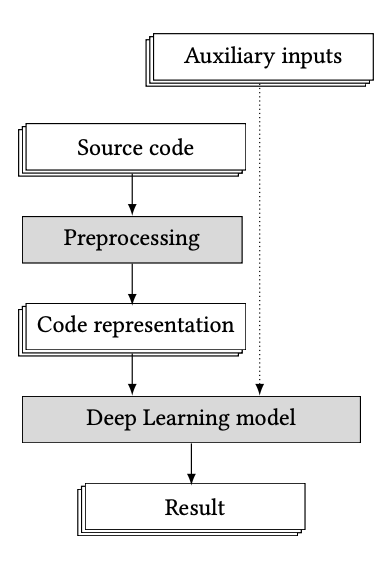
\includegraphics[width=2.5cm, height=3.5cm]{figures/high_level_prediciton_task.png}
    \caption{\cite{compiler_based} High level overview of the function classification preditction task.}
    \label{fig:predictive_task}
\end{figure}

We utilized various 
types of representations of single function's raw source code to provide the models with data.
These include word tokenized TF-IDF vectors for Random Forests, BPE of raw source code for
BERT, linearized AST pre-order traversal for BERT and representation set of randomly selected 600 node-to-node paths for AttentionNN.  
PsycheC project's C language frontend parser \cite{psychec} was used for parsing the code into ASTs. Each model was trained in Tensorflow.Keras framework and with different author set sizes to evaluate scalabillity. The different set sizes were
110, 27, 11, 3 with each having increased demands on minimal function count than the one before. The minimal function counts per author for the sizes were 25, 40, 50, 58 respectively.

\subsection{Data preprocessing \& Exploratory data analysis}
The dataset consisted of thousands of solutions from hundreds of authors. From each solution we extracted the function and its author.
The largest of the different sized datasets we used consisted of $3\,004$ C language functions' source code gathered from Google Code Jam (GCJ) solutions from years 2009 to 2018. The data was preprocessed exclude duplicates, 
remove outlying authors that have multiple times more samples than is the average number of samples per author to reduce the models' bias towards these names. Functions 
that could not be parsed into an AST were also eliminated to ensure consistency in the datasets. This allows for a fair assessment of each model, 
as they utilize different representations of function data. For further analysis, we needed to see the frequency distributions of authors. 


\begin{figure}[h]
    \centering
    \begin{subfigure}{0.48\textwidth} % Adjust width to fit
        \centering
        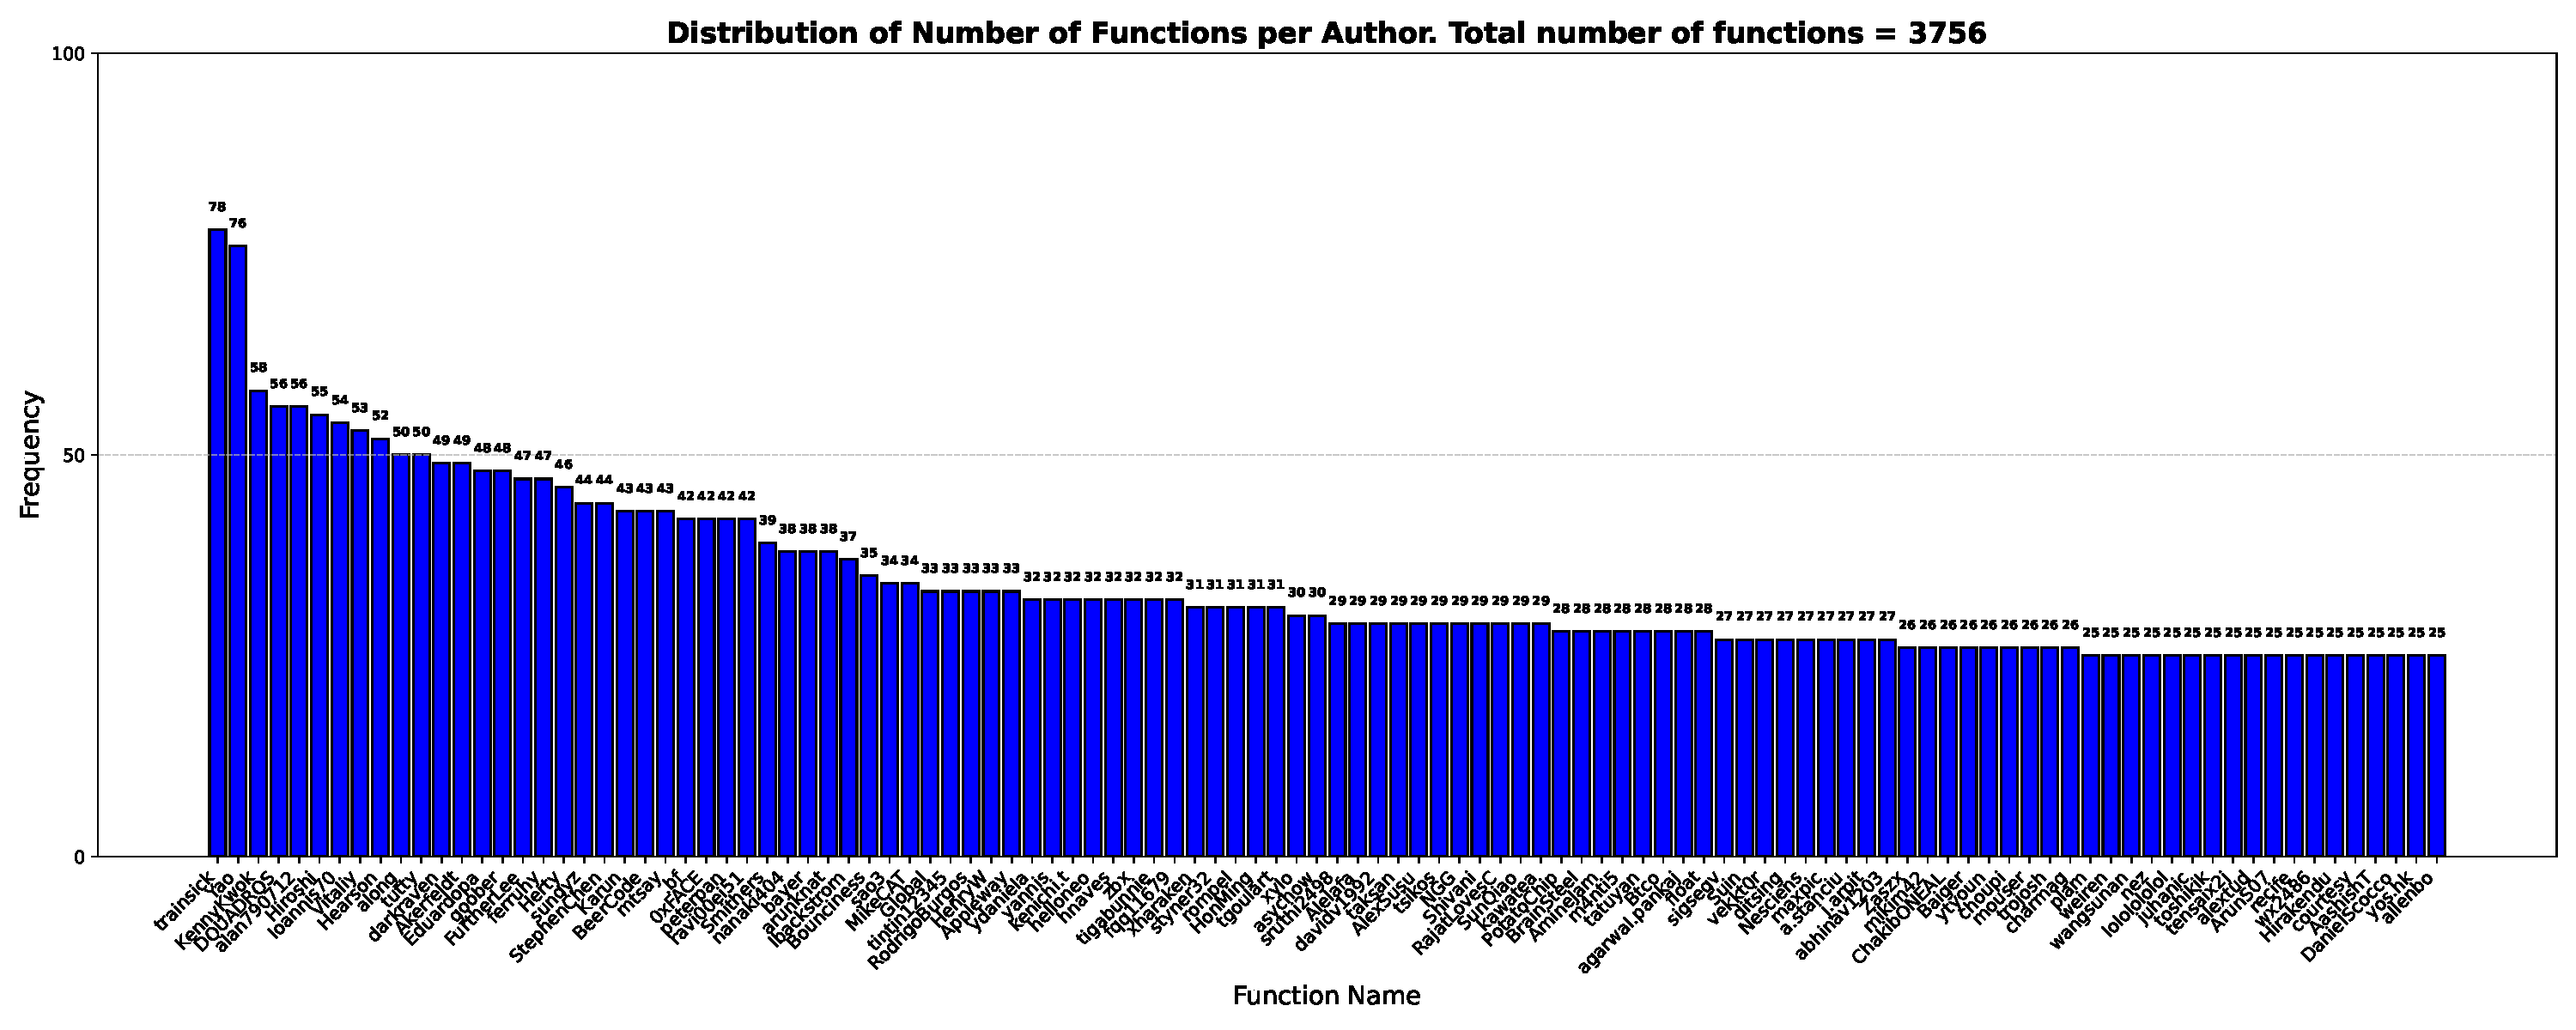
\includegraphics[width=\linewidth]{figures/distribution_names.pdf}
        \caption{Frequency distribution of author names}
        \label{fig:distr_names}
    \end{subfigure}
    \hfill
    \begin{subfigure}{0.48\textwidth}
        \centering
        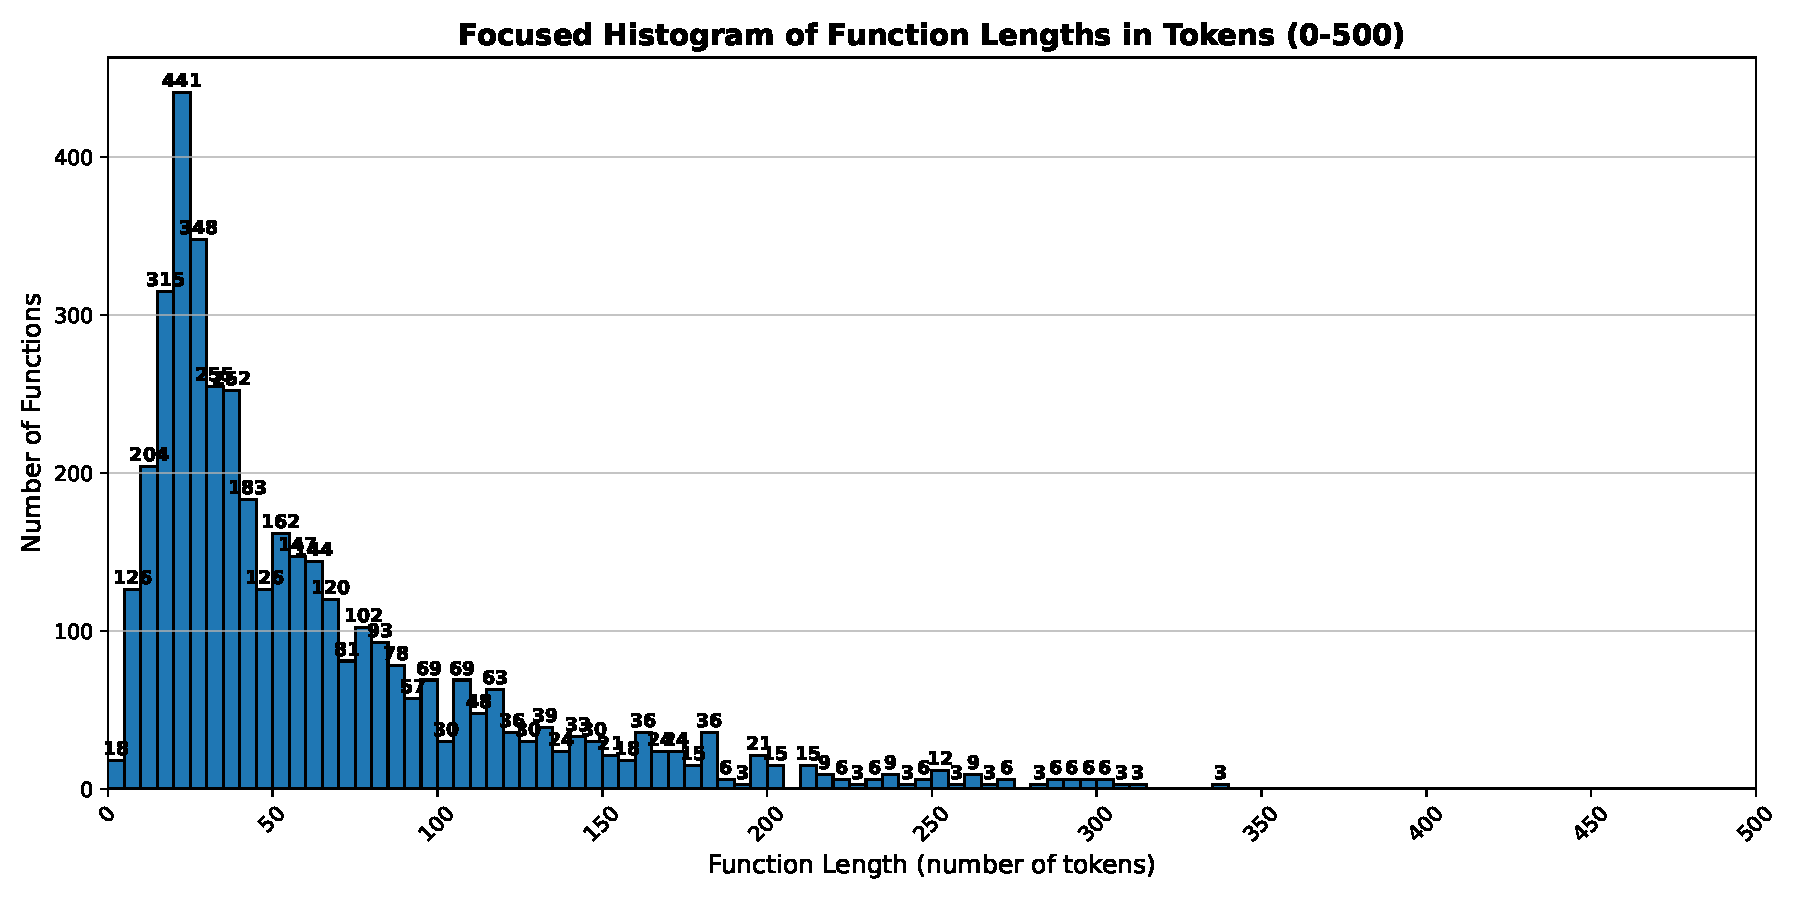
\includegraphics[width=\linewidth]{figures/distr_lens_tokens.pdf}
        \caption{Frequency distribution of function lengths}
        \label{fig:disrt_lens}
    \end{subfigure}
    \caption{Important frequency distributions of our dataset}
    \label{fig:eda_distr}
\end{figure}

From the figure \ref{fig:distr_names} we can see that the most of our dataset's 
functions lengths lie between 10 and 50 tokens which makes our goal of authorship attribution of single function
harder than if given a whole file consisting of multiple functions or code blocks in sense that for the prediction
most of the time we only have from 10 to 50 tokens available to find the correct author.

\section{Models setup \& training}

In this section we will discuss the training strategies and setup for the examined models.
Random Forests and AttentionNN models were trained using Stratified Cross validation strategy that ensures, that each author is evenly distributed
across the folds. Number of folds was set to 5 and 3 folds were used for training, 1 for validation and 1 for testing.
As training of BERT takes a lot more time than the other 2, we just repeated the traing 3 times and 
observed variance in evaluation metrics lower than 1\%.

\subsection{Random Forests}

For comparison purposes, we have chosen Random Forests as standard approach to text based authorship attribution. 
They were trained on word-level tokens using the regex pattern \verb|r"\b\w+\b"|, which matches words separated by word boundary characters.
Firt we used grid search to optimize these hyperparameters:
\begin{itemize}
    \item \textbf{n\_estimators}: \{50, 100, 200, 500\}
    \item \textbf{max\_depth}: \{10, 20, 30, None\}
    \item \textbf{min\_samples\_split}: \{2, 5, 10\}
    \item \textbf{min\_samples\_leaf}: \{1, 2, 4\}
    \item \textbf{max\_features}: \{"sqrt", "log2", None\}
    \item \textbf{bootstrap}: \{True, False\}
\end{itemize}

and then we trained the model using the best hyperparameters found.

\subsection{BERT}

For both BERT training setups we used Microsoft's pretrained graphcodebert-base \cite{codebert} that already understands general programming concepts like 
control structures, loops or functions and is able to capture differences between authors faster. We also used the graphcodebert tokenizer which uses 
Byte pair encoding that merges frequently occurring character sequences into tokens, which is appropriate for data like source code of programming language
that has very rigid syntax. The comments in all code samples were filtered out so the attribution task
is 'fair' across the models that utilize ASTs.

As mentioned, we have trained the BERT model on two distinct data representations. Tokenized RAW source code and tokenized AST pre-order traversal
to see how the model reacts to these representations and how useful it may be to learn from the AST structural patterns in comparison to AttentionNN 
that utilizes node-to-node paths.

\subsection{Attention Neural Network}

To capture all three of the structural, semantic and syntactic features in a number vector that could be somehow fed into a neural network classifier. 
Code2vec \cite{code2vec} proposes solution design that extracts so called 'path-contexts' which are encoded into vector space using the embedding values 
of its components.
Path-contexts capture the node-to-node path in concise manner as it consist of triplets of <start node, the path of nodes kinds, terminal node>.
Each distinct node is encoded with the data value it carries and each distinct path is encoded as a string of nodes' kinds in between the start and terminal node.
The model then learns to distinguish the authors utilizing the attention mechanism, giving larger weights to contexts that help to reveil the author the most.

\subsection{Evaluation methods}
For evaluation purposes metrics such as validation Accuracy, Precision, Recall, Time to train model and Halstead complexity measures were captured to explain the models
behavior with different kinds of data. The deep-learning models were trained with the Categorical Cross-Entropy loss function guiding the optimization process,

\begin{equation}
    \mathcal{L}_i = - \sum_{j=1}^{C} y_{i,j} \log(\hat{y}_{i,j})
\end{equation}

where:
\begin{itemize}
    \item $\mathcal{L}_i$ is the loss for the $i$-th sample.
    \item $C$ is the number of possible classes.
    \item $y_{i,j}$ represents the ground truth label for class $j$. It is a one-hot encoded vector, meaning:
    \begin{itemize}
        \item $y_{i,j} = 1$ if the sample belongs to class $j$.
        \item $y_{i,j} = 0$ otherwise.
    \end{itemize}
    \item $\hat{y}_{i,j}$ is the predicted probability for class $j$, obtained from a softmax function.
    \item $\log(\hat{y}_{i,j})$ takes the logarithm of the predicted probability.
\end{itemize}

We also looked at the learning curves of the deep leaning models (BERT, AttentionNN) to assess the overfit of each one and compared the models in terms of 
accuracy for functions of different complexity obtaining interesting results revealing their strengths and weaknesses.


\section{Results}

As we have mentioned, the models were mainly tested for their scalability with having more functions per author while decreasing the distinct author set size.
The following table \ref{tab:comparison} summarizes how each model performed in terms of accuracy and the time required for training (until the validation loss stopped decreasing) across diverse datasets
and figure \ref{fig:3d-bars} visualizes the achieved performances on Accuracy, Precision and Recall. From table \ref{tab:comparison} we can say that BERT 
trained on tokens extracted from the raw source code performed the best at each of the author set sizes, especially with accuracy over 90\% on the smallest set, however with the longest required time to train the model, more than 
9.5 times longer than it took to train AttentionNN to its full potential and 36.4 times longer than the time required for Random Forests which scored just 4.8 percent less.
What also interested us is that From \texttt{set\_size=11} to \texttt{set\_size=3}, BERT improved only by 0.86\% which is the smallest improvement across all the experiments and indicates that increasing the minimum function 
count per author from 50 to 58 had little impact on the model's ability to distinguish authors. 
On the other hand, from being the worst, BERT fed with AST pre-order traversal scored a 40\% higher under these conditions. 

\begin{table}[H]
    \centering
    {\scriptsize
    \begin{tabular}{lcccc}
    \hline
    \multicolumn{5}{c}{\textbf{Models' Author Attribution Accuracy for Different Author Set Sizes}} \\
    \hline
    \textbf{Model} & \multicolumn{4}{c}{\textbf{Author Set Size}} \\
    \cline{2-5}
                  & 110  & 27  & 11 & 3 \\ 
    \hline
    Random Forests (TF--IDFs w/o comments) & 66.24\%\;|\;$3.63\,\mathrm{min}$ & 70.60\%\;|\;$0.23\,\mathrm{min}$ & 80.56\%\;|\;$0.08\,\mathrm{min}$ & 85.84\%\;|\;$0.05\,\mathrm{min}$ \\
    BERT (source code w/o comments)        & 72.47\%\;|\;$30.33\,\mathrm{min}$ & 82.72\%\;|\;$9.49\,\mathrm{min}$ & 89.84\%\;|\;$5.3\,\mathrm{min}$  & \textbf{90.70\%\;|\;\boldmath$1.82\,\mathrm{min}$}\\
    BERT (AST pre\_order traversal)        & 24.07\%\;|\;$33.53\,\mathrm{min}$ & 35.66\%\;|\;$10.3\,\mathrm{min}$ & 40.62\%\;|\;$6.2\,\mathrm{min}$  & 83.72\%\;|\;$1.22\,\mathrm{min}$ \\
    AttentionNN (AST NtN paths)            & 36.93\%\;|\;$3.53\,\mathrm{min}$ & 53.42\%\;|\;$1.19\,\mathrm{min}$ & 60.82\%\;|\;$0.54\,\mathrm{min}$  & 69.3\%\;|\;$0.19\,\mathrm{min}$ \\
    \hline
    \end{tabular}
    }
    \caption{Comparison of models across author attribution accuracy and training time for different author set sizes.}
    \label{tab:comparison}
\end{table}

\begin{figure}[H] 
    \centering
    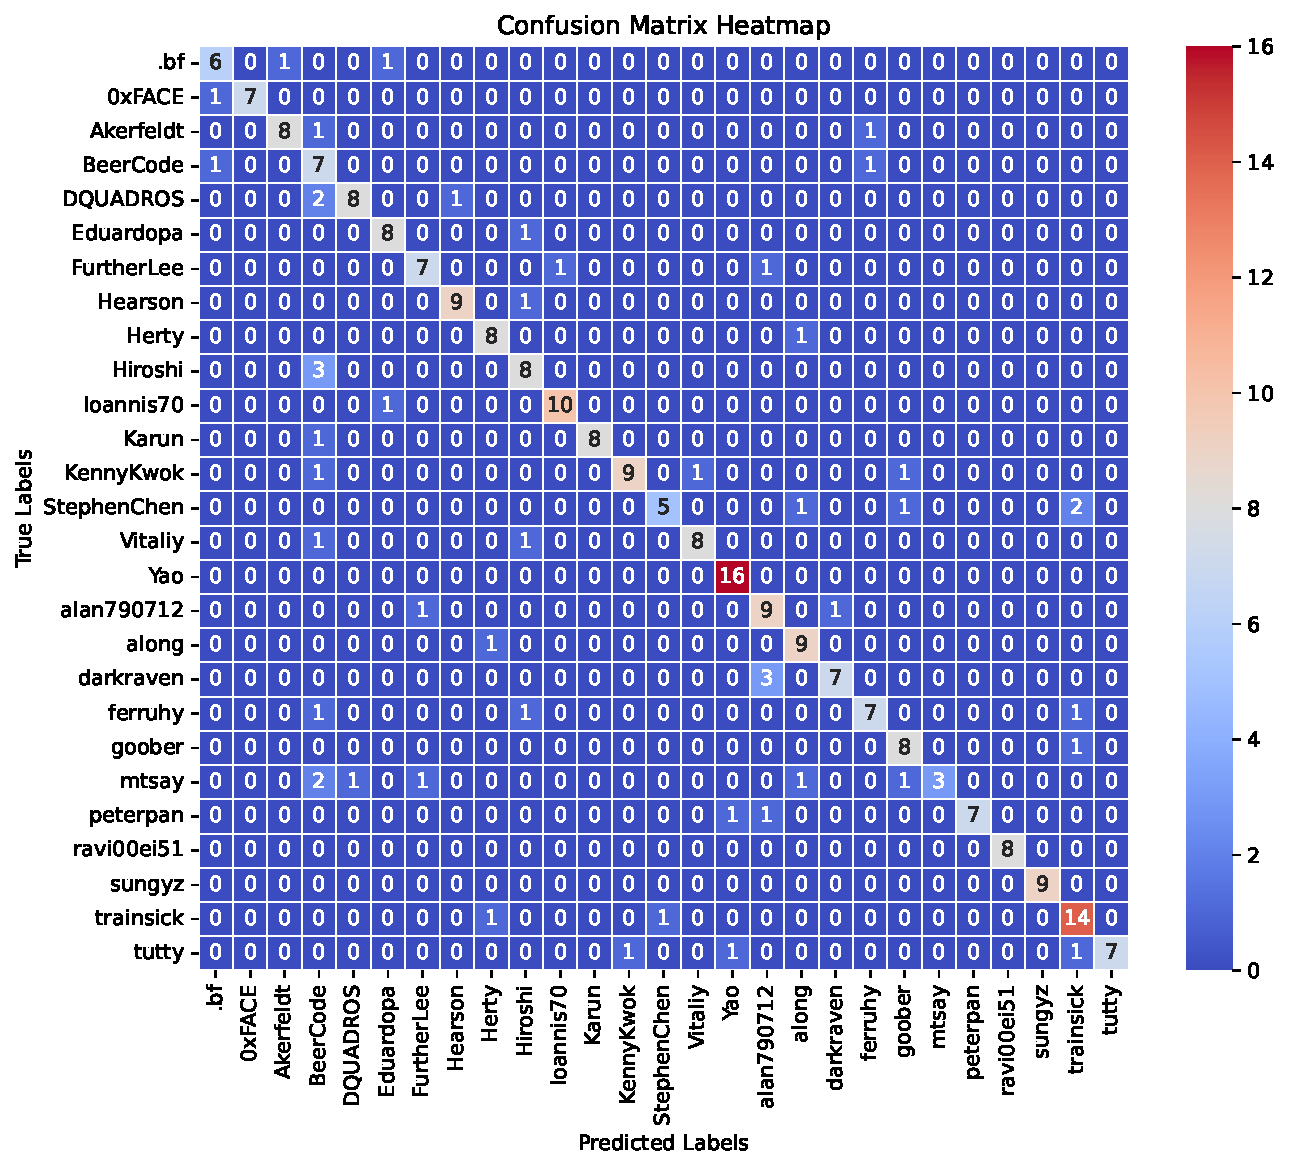
\includegraphics[width=0.6\textwidth]{figures/conf_matrix_sourcode_bert_ts27.pdf}
    \caption{Confusion matrix for best performative model BERT trained on author set of size 27.}
    \label{fig:conf_matrix_bert}
\end{figure}

The confusion matrix shows, that the model performed best on 2 most represented authors
(see \ref{fig:distr_names}). Although if we take 8 most represented authors, only 5 of them are also 
the most accurately classified.


In terms of overfit BERT with tokenized source codes was able to generalize the datasets in effective manner reaching 1.41, 1.24, 1.05, 1.12 for overfit ratios 
calculated like this

\begin{equation}
    \text{Overfit Ratio} = \frac{\text{Train Accuracy}}{\text{Test Accuracy}}
\end{equation}

and only the latter two are under the limit of 1.2 - being optimally fitted. 

Random forests reached 1.51, 1.3, 1.24, 1.15 overfit ratios which still show a considerable amount of generalization. However AttentionNN was not that successful with generalizing 
and with the dataset consisting of 3 distinct authors it got overfit of 1.4 and only increasing with each larger dataset, meaning insufficient data is being provided for the network so it starts memorizing particular 
patterns instead of actually generalizing above authors, which does not allow the model to perform better on unseen data affecting its validation accuracy.

\begin{figure}[H]
\centering
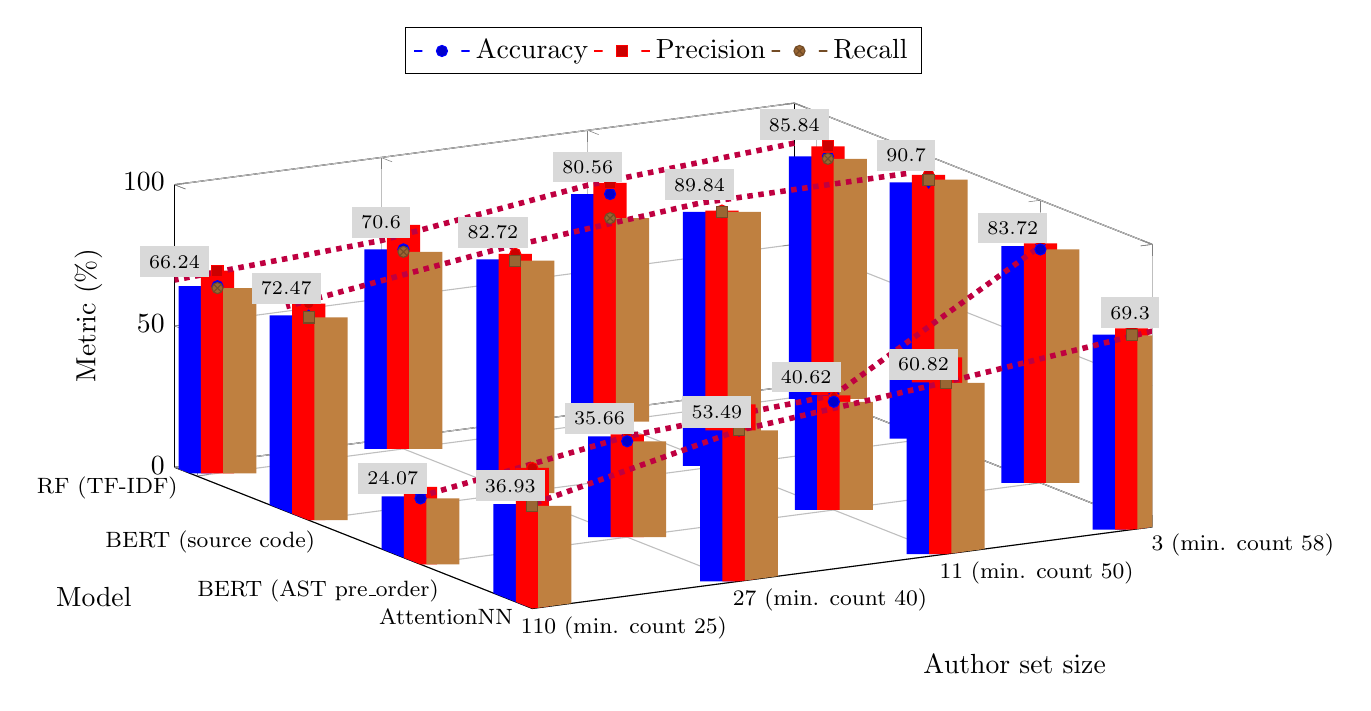
\begin{tikzpicture}
\begin{axis}[
    view={60}{30},            % 3D viewing angles (azimuth, elevation)
    z buffer=sort,            % Ensures correct front-to-back rendering
    xlabel={Model},
    xlabel style={
        xshift = -40pt,
        yshift=40pt,
        align=center          % optional alignment
    },
    ylabel={Author set size},
    ylabel style={
        xshift = 25pt,
        yshift=20pt,
        align=center          % optional alignment
    },
    zlabel={Metric (\%)},
    width=14cm,
    height=8cm,
    xtick={1,2,3,4},
    xticklabels={RF (TF-IDF), BERT (source code), BERT (AST pre\_order), AttentionNN},
    xticklabel style={
        font=\footnotesize,    % or \footnotesize, \tiny, etc.
        xshift = -20pt,
        yshift=10pt,
        align=center          % optional alignment
    },
    ytick={4,3,2,1}, % Reversed ytick values
    yticklabels={3 (min. count 58), 11 (min. count 50), 27 (min. count 40), 110 (min. count 25)}, % Corresponding reversed labels
    yticklabel style={
        font=\footnotesize,    % or \footnotesize, \tiny, etc.
        xshift = 25pt,
        yshift=5pt,
        align=center          % optional alignment
    },
    zmin=0, zmax=100,
    grid=major,
    legend style={
        at={(0.5,1.15)},
        anchor=north,
        legend columns=3
    }
]

%%%%%%%%%%%%%%%%%%%%%%%%%%%%%%%%%%%%%%%%%%%%%%%%%%%%%%%%%%%%%%
% MODEL 1: RF (x = 1)
%%%%%%%%%%%%%%%%%%%%%%%%%%%%%%%%%%%%%%%%%%%%%%%%%%%%%%%%%%%%%%

\addplot3+[ybar, bar width=12pt, fill=blue, draw=none, bar shift=-0.2]
    coordinates {(1.1,4,85.84) (1,3,80.56) (1,2,70.60) (1,1.1,66.24)}; % Coordinates are adjusted to match the reversed ytick
\addplot3+[ybar, bar width=12pt, fill=red, draw=none, bar shift=0]
    coordinates {(1.1,4,89.36) (1,3,84.56) (1,2,79.27) (1,1.1,71.73)}; % Coordinates are adjusted to match the reversed ytick
\addplot3+[ybar, bar width=12pt, fill=brown, draw=none, bar shift=+0.2]
    coordinates {(1.1,4,84.96) (1,3,72.03) (1,2,69.73) (1,1.1,65.55)}; % Coordinates are adjusted to match the reversed ytick

    %dotted line
\addplot3+[
    mark=none,
    purple,
    dotted,
    line width=2pt,
    nodes near coords,
    every node near coord/.append style={
        mark=none,
        fill=gray!30,
        draw=none,
        text=black,
        font=\scriptsize,
        yshift=0pt
    }
] coordinates {
    (0.8,4,85.84) (0.8,3,80.56) (0.8,2,70.60) (0.8,1,66.24) % Coordinates are adjusted to match the reversed ytick
};

%%%%%%%%%%%%%%%%%%%%%%%%%%%%%%%%%%%%%%%%%%%%%%%%%%%%%%%%%%%%%%
% MODEL 2: BERT-SOURCE (x = 2)
%%%%%%%%%%%%%%%%%%%%%%%%%%%%%%%%%%%%%%%%%%%%%%%%%%%%%%%%%%%%%%

\addplot3+[ybar, bar width=12pt, fill=blue, draw=none, bar shift=-0.2]
    coordinates {(2,4,90.70) (2,3,89.84) (2,2,82.72) (2,1,72.47)}; % Coordinates are adjusted to match the reversed ytick
\addplot3+[ybar, bar width=12pt, fill=red, draw=none, bar shift=0]
    coordinates {(2,4,93.33) (2,3,90.33) (2,2,84.66) (2,1,76.69)}; % Coordinates are adjusted to match the reversed ytick
\addplot3+[ybar, bar width=12pt, fill=brown, draw=none, bar shift=+0.2]
    coordinates {(2,4,91.67) (2,3,89.92) (2,2,82.25) (2,1,71.76)}; % Coordinates are adjusted to match the reversed ytick

\addplot3+[
    mark=none,
    purple,
    dotted,
    line width=2pt,
    nodes near coords,
    every node near coord/.append style={
        mark=none,
        fill=gray!30,
        draw=none,
        text=black,
        font=\scriptsize,
        yshift=0pt
    }
] coordinates {
    (1.8,4,90.70) (1.8,3,89.84) (1.8,2,82.72) (1.8,1,72.47) % Coordinates are adjusted to match the reversed ytick
};

%%%%%%%%%%%%%%%%%%%%%%%%%%%%%%%%%%%%%%%%%%%%%%%%%%%%%%%%%%%%%%
% MODEL 3: BERT-AST (x = 3)
%%%%%%%%%%%%%%%%%%%%%%%%%%%%%%%%%%%%%%%%%%%%%%%%%%%%%%%%%%%%%%

\addplot3+[ybar, bar width=12pt, fill=blue, draw=none, bar shift=-0.2]
    coordinates {(3,4,83.72) (3,3,40.62) (3,2,35.66) (3,1,24.07)}; % Coordinates are adjusted to match the reversed ytick
\addplot3+[ybar, bar width=12pt, fill=red, draw=none, bar shift=0]
    coordinates {(3,4,84.72) (3,3,40.53) (3,2,36.41) (3,1,27.40)}; % Coordinates are adjusted to match the reversed ytick
\addplot3+[ybar, bar width=12pt, fill=brown, draw=none, bar shift=+0.2]
    coordinates {(3,4,82.58) (3,3,38.30) (3,2,33.93) (3,1,23.33)}; % Coordinates are adjusted to match the reversed ytick
\foreach \yA/\zA/\yB/\zB in {
    4/83.72/3/40.62,
    3/40.62/2/35.66,
    2/35.66/1/24.07
} {
    \addplot3+[
        mark=none,
        purple,
        dotted,
        line width=2pt,
        nodes near coords,
        every node near coord/.append style={
            mark=none,
            fill=gray!30,
            draw=none,
            text=black,
            font=\scriptsize,
            yshift=0pt,
            xshift=-10pt
        }
    ] coordinates {
        (3,\yA,\zA) (3,\yB,\zB)
    };
}

%%%%%%%%%%%%%%%%%%%%%%%%%%%%%%%%%%%%%%%%%%%%%%%%%%%%%%%%%%%%%%
% MODEL 4: ATTENTION-NN (x = 4) - Data missing => set to 0
%%%%%%%%%%%%%%%%%%%%%%%%%%%%%%%%%%%%%%%%%%%%%%%%%%%%%%%%%%%%%%
\addplot3+[ybar, bar width=12pt, fill=blue, draw=none, bar shift=-0.2]
    coordinates {(4,3.9,69) (4,3,60.82) (4,2,53.42) (4,1,36.93)}; % Coordinates are adjusted to match the reversed ytick
\addplot3+[ybar, bar width=12pt, fill=red, draw=none, bar shift=0]
    coordinates {(4,3.9,71.25) (4,3,69.6) (4,2,62.6) (4,1,49.73)}; % Coordinates are adjusted to match the reversed ytick
\addplot3+[ybar, bar width=12pt, fill=brown, draw=none, bar shift=+0.2]
    coordinates {(4,3.9,68.76) (4,3,60.61) (4,2,53.45) (4,1,36.34)}; % Coordinates are adjusted to match the reversed ytick
\foreach \yA/\zA/\yB/\zB in {
    4/69.3/3/60.82,
    3/60.82/2/53.42,
    2/53.49/1/36.93
} {
    \addplot3+[
        mark=none,
        purple,
        dotted,
        line width=2pt,
        nodes near coords,
        every node near coord/.append style={
            mark=none,
            fill=gray!30,
            draw=none,
            text=black,
            font=\scriptsize,
            yshift=0pt,
            xshift=-8pt
        }
    ] coordinates {
        (4,\yA,\zA) (4,\yB,\zB)
    };
}

%%%%%%%%%%%%%%%%%%%%%%%%%%%%%%%%%%%%%%%%%%%%%%%%%%%%%%%%%%%%%%
% LEGEND
%%%%%%%%%%%%%%%%%%%%%%%%%%%%%%%%%%%%%%%%%%%%%%%%%%%%%%%%%%%%%%
\addplot3[
    ybar, 
    fill=blue, 
    draw=none, 
    bar width=12pt, 
    legend image code/.code={
        \draw[fill=blue] (0cm,-0.1cm) rectangle (0.6cm,0.1cm);
    }
] coordinates {(0,0,-9999)};
\addlegendentry{Accuracy}

\addplot3[
    ybar, 
    fill=red, 
    draw=none, 
    bar width=12pt, 
    legend image code/.code={
        \draw[fill=red] (0cm,-0.1cm) rectangle (0.6cm,0.1cm);
    }
] coordinates {(0,0,-9999)};
\addlegendentry{Precision}

\addplot3[ % Recall
    ybar, 
    fill=brown, 
    draw=none, 
    bar width=12pt, 
    legend image code/.code={
        \draw[brown, mark=x] plot coordinates {(0cm,0cm)}; 
    }
] coordinates {(0,0,-9999)};
\addlegendentry{Recall} 

\end{axis}
\end{tikzpicture}
\caption{Bar chart comparing Accuracy (with accuracy values labeled), Precision, and Recall across models and author set sizes with minimum function count per author. }
\label{fig:3d-bars}
\end{figure}

\subsection{Comparing models' performance depending on the complexity of function}

In our task of identifying an author given a single function, a natural question arises: how did the models 
perform on functions of different complexities? The basic indicator of function complexity is its length. So we came up with strategy, 
how to visually compare models, even when the number of each model's misclassifications is different. We scaled the models histogram bin values by 
an index that is obtained like this: 

\begin{equation}
    \text{index}_{i} = \frac{\text{Number of misclassifications of the worst performative model}}{\text{Number of misclassifications of model}_{i}}
\end{equation}

This way we obtain visual representation that objectively accounts for the fact that the number of errors is different.
In the following figure we visualized the frequencies of misclassified function lengths in tokens for Random Forests, BERT and AttentionNN scaling each 
model with its index.


\begin{figure}[H] 
    \centering
    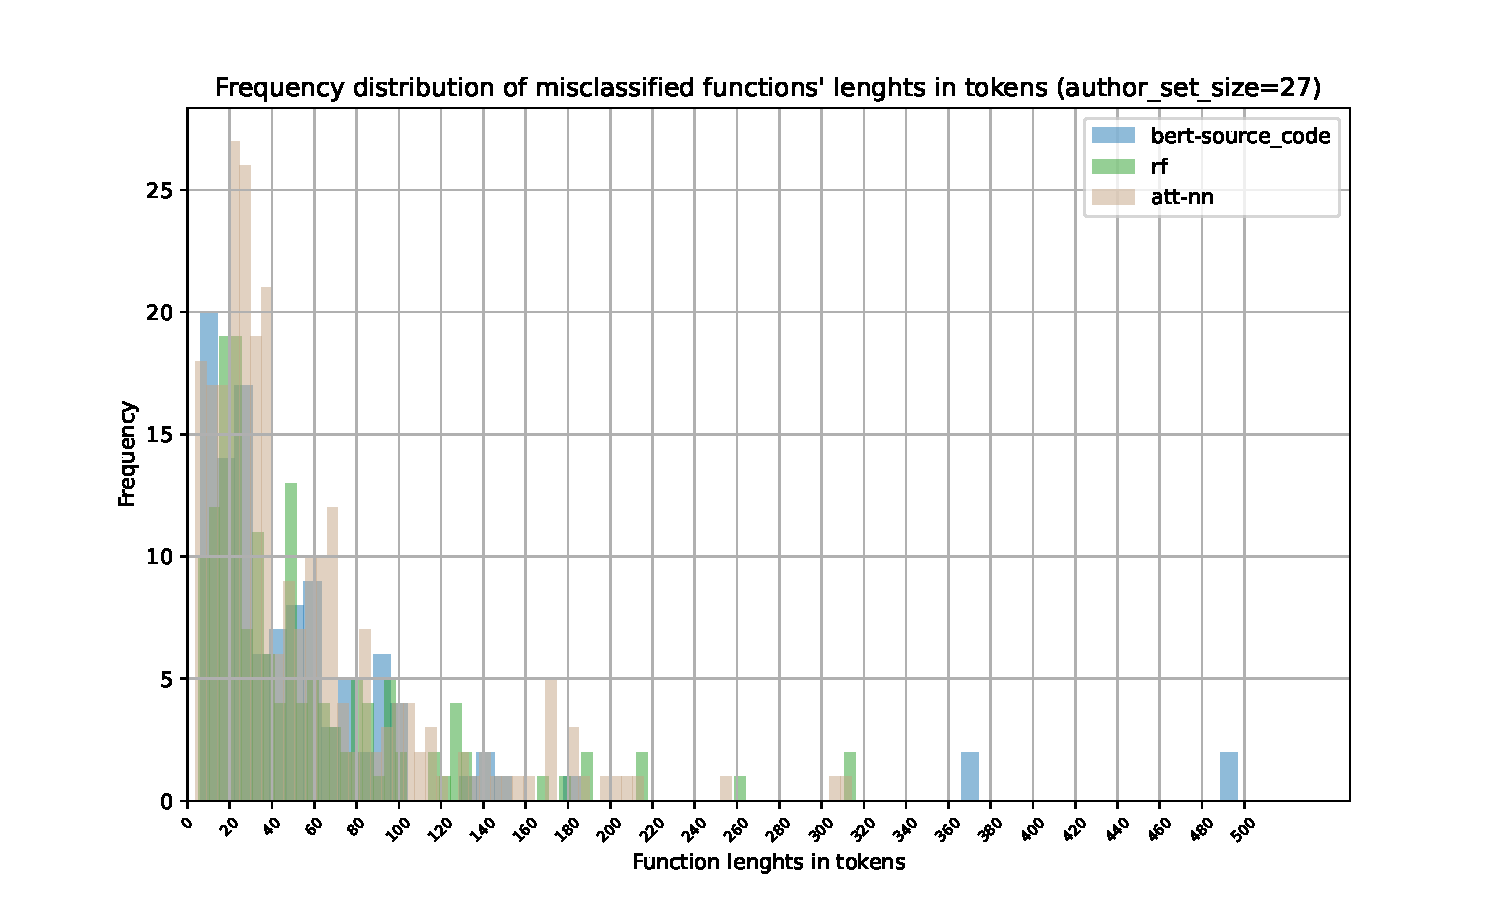
\includegraphics[width=0.8\textwidth]{figures/misclass_lens.pdf}
    \caption{The frequency distribution of misclassified function lengths in tokens for Random Forests, BERT and AttentionNN}
    \label{fig:misclass_lens}
\end{figure}

From the figure \ref{fig:misclass_lens} the only statement we can say is that the model AttentionNN particularly struggled with functions of length lower than 40 tokens
but did quite well on the longer ones. This will be discussed in the following subsection more deeply \ref{subsec:comp_over_quant}.
Other models performance is not really distinguishable from this visualization, so we performed the same index strategy with the Halstead complexity metrics.
Measuring each misclassified function's Halstead complexity and plotting it for Random Forests and BERT trained on tokenized source code, we obtained following figure.

\begin{figure}[H] 
    \centering
    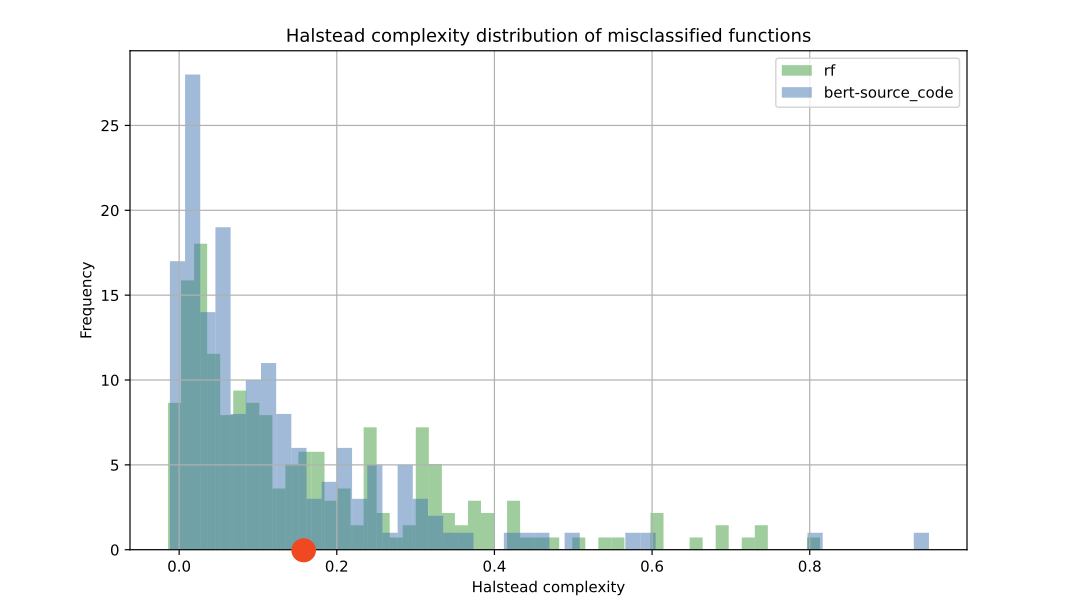
\includegraphics[width=0.8\textwidth]{figures/misclass_hs.png}
    \caption{The frequency distribution of misclassified function Halstead complexity for Random Forests and BERT.}
    \label{fig:misclass_halstead}
\end{figure}

This error distribution reveals that Random Forests struggled more with Halstead complexity increasing from the marked red point compared to the BERT 
Specifically there are 1.59 times more misclassifications made by the Random Forest classifier than there are by BERT measured from the red point.
However, closer we look to 0 on x axis, the more errors we see made by BERT. This would be the main difference between the deep learning and 
machine learning method. The deep learning method utilizes self-attention that enables it to capture more complex relationships but struggles
to categorize when limited or not complex enough data is provided, not being able to find the relationships that characterize the author of the function. 
On the other hand, the machine learning TF-IDF method struggles with the more complex data because the representation lacks context understanding and solely 
relies on the number of occurrences in the sample.

\subsection{Attention neural network - complexity over quantity}  \label{subsec:comp_over_quant}

Considering the observation in figure \ref{fig:misclass_lens}, where AttentionNN performed worst on lengths between 20 and 40 tokens,
we assesed the model in a deeper manner. Evaluating accuracies across functions distributed into bins according to 2 metrics. 
Number of nodes in the AST and depth of the AST of the function. 

\begin{figure}[H]
    \centering
    \begin{subfigure}{0.48\textwidth} 
        \centering
        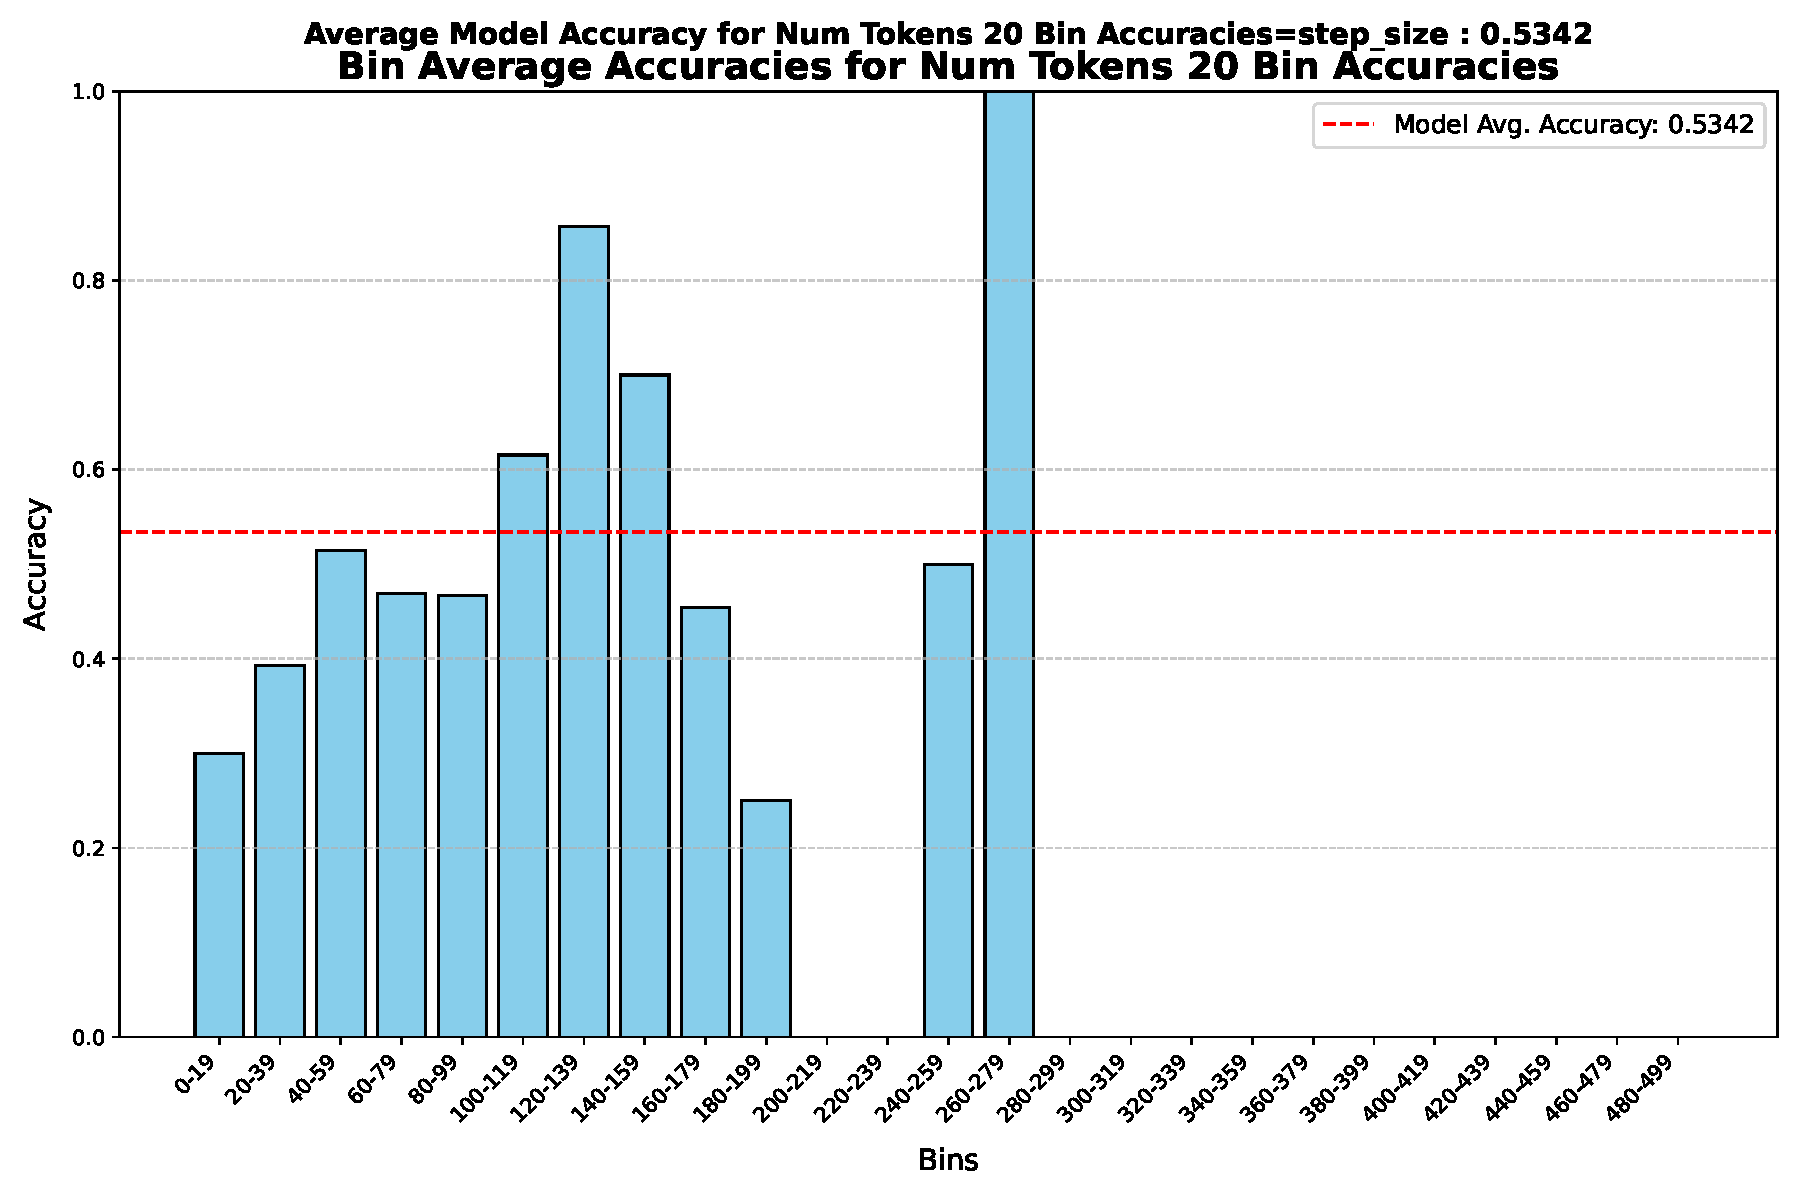
\includegraphics[width=\linewidth]{figures/attention_nn/ann_acc_num_nodes.pdf}
        \caption{Accuracy across different bins of number of nodes in function's AST}
        \label{fig:distr_names}
    \end{subfigure}
    \hfill
    \begin{subfigure}{0.48\textwidth}
        \centering
        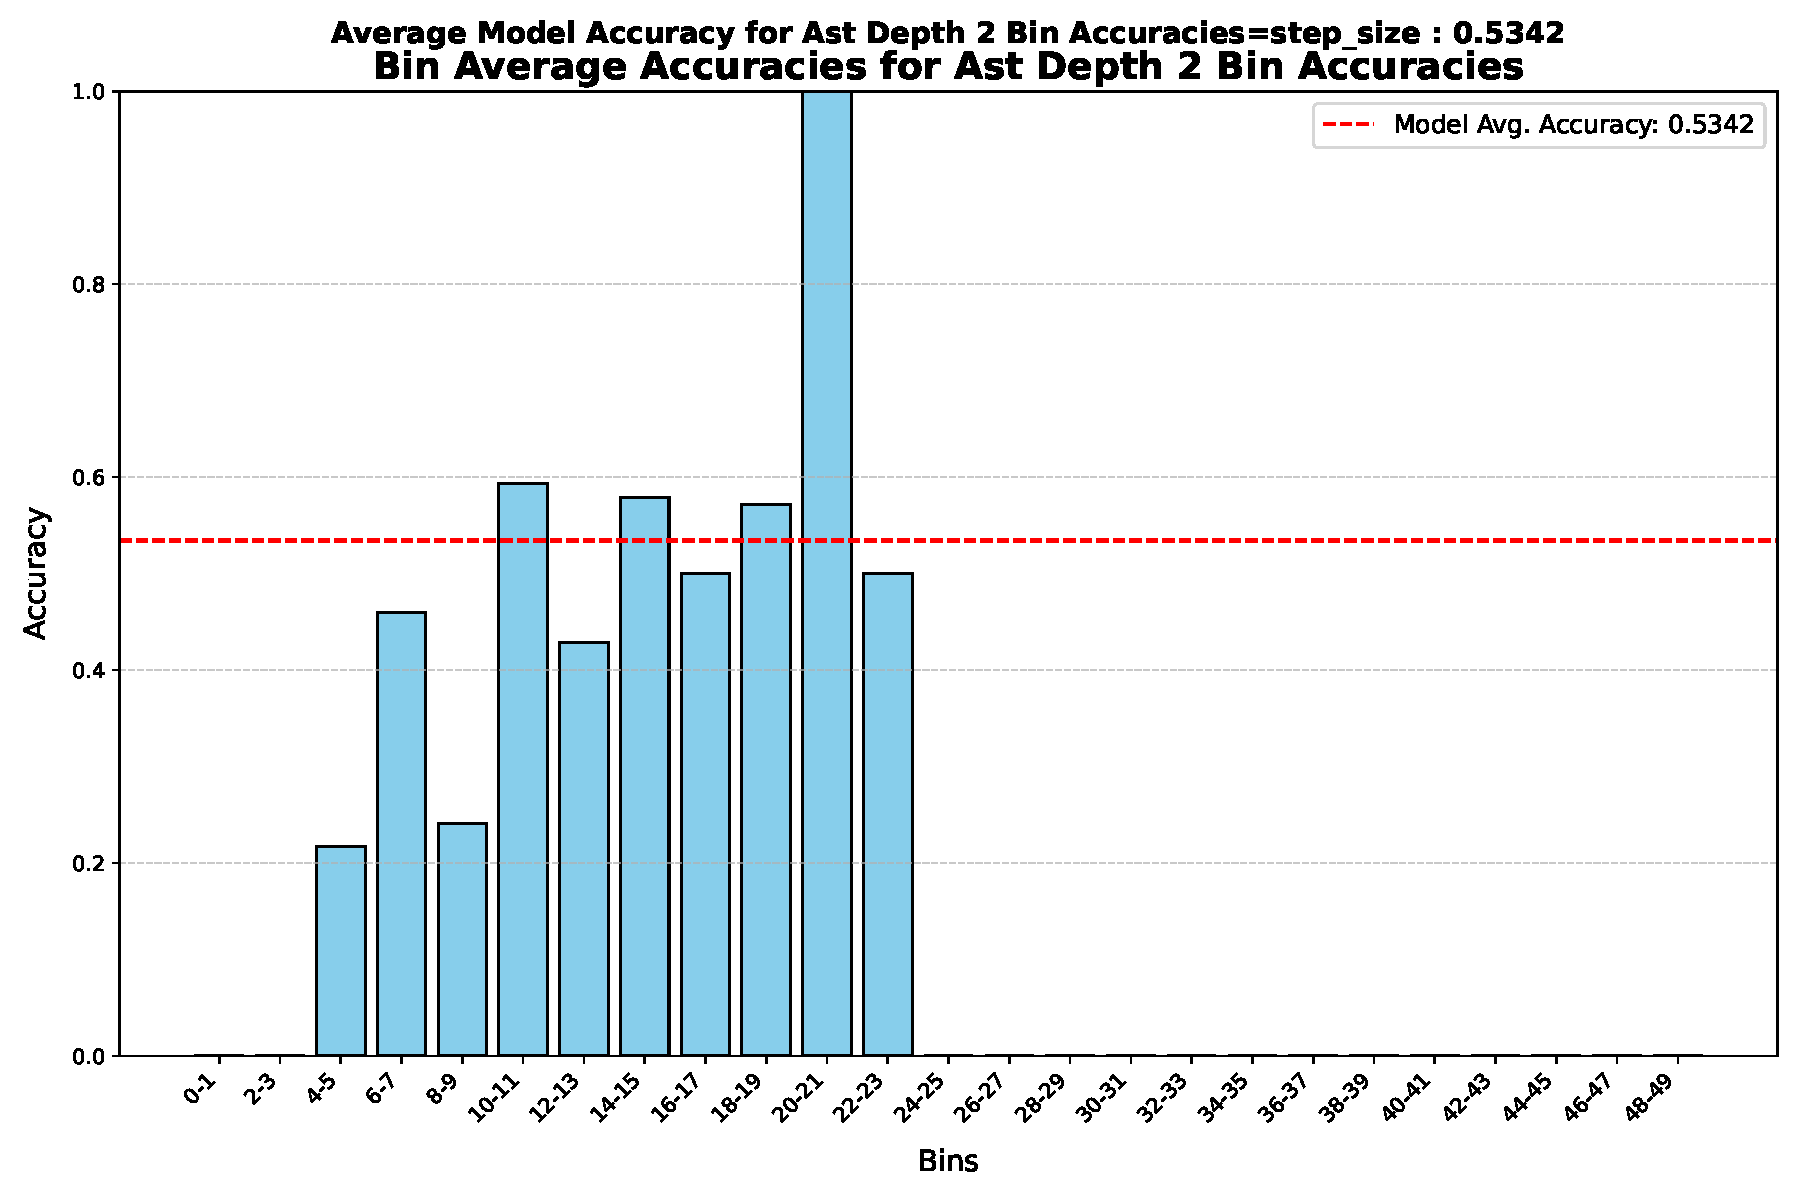
\includegraphics[width=\linewidth]{figures/attention_nn/ann_acc_depth.pdf}
        \caption{Accuracy across different bins of depth in function's AST}
        \label{fig:disrt_lens}
    \end{subfigure}
    \caption{AttNN Accuracy of functions with different complexities}
    \label{fig:eda_distr}
\end{figure}

From the figure we can deduce, there is an emerging trend in accuracy from bins of lower value to the bins of higher value.
Eventhough the frequency distribution of both variables indicates more frequency on the lower values we observe a lower
accuracy. This tells that the model is learning rather from more structural complex functions than simple non-nesting and 
control-flow divergent ones.

\section{Discussion}

Our findings show that deep learning models, especially BERT, perform better than traditional machine learning methods for authorship attribution 
of single functions. But this comes at a cost—BERT needs way more computation and training time. On the other hand, Random Forest with TF-IDF 
tokenization held up surprisingly well, especially with larger author sets, and trained very fast.

A key takeaway is that BERT trained on raw source code tokens consistently had the best accuracy across all dataset sizes. However, 
its improvement from \texttt{set\_size=11} to \texttt{set\_size=3} was only 0.86\%, meaning increasing the minimum function count per author 
after a certain point doesn’t do much. Interestingly, BERT using AST pre-order traversal struggled with large author sets but got way better 
when we reduced the dataset to three authors. This shows how important it is to choose the right input representation for deep learning models.

Looking at misclassifications, each model had its weak points. BERT had trouble with short functions that had low Halstead complexity— they 
don’t provide enough meaningful context to determine the author. Random Forests, which rely more on statistical patterns than contextual 
understanding, started failing as function complexity increased. This makes sense since TF-IDF representations capture token frequency but 
don’t really understand code structure.

AttentionNN, which works with AST-derived node-to-node paths, preferred structurally complex functions over simple ones. This means that 
networks using structural information may do better with more complex functions rather than short, flat ones. However, AttentionNN didn’t 
generalize well when data was limited, and it started overfitting when trained on small author sets. This shows we either need bigger 
datasets or more regularization to prevent overfitting.

The results highlight a clear trade-off between model complexity, training time, and accuracy. Deep learning models, while powerful, 
require serious computational resources, making them harder to scale in real-world use cases. Random Forests might not be as accurate, 
but they’re super efficient and a solid alternative when speed is a concern.

Going forward, it would be interesting to combine these methods. For example a hybrid approach using BERT embeddings with Random Forest 
classifier could balance accuracy and efficiency. Also, using graph-based neural networks to process ASTs more effectively might push 
authorship attribution even further. Exploring data augmentation techniques or better regularization strategies could also help deep 
learning models generalize better, especially with AST-based inputs.

\section{Conclusion}

In this study, we compared traditional machine learning models and deep learning models for authorship attribution of individual functions. 
Our results showed that while BERT-based models provided the highest accuracy, they required significantly longer training times and 
computational resources. In contrast, Random Forests trained on TF-IDF representations performed surprisingly well given their simplicity 
and efficiency.

The choice of model largely depends on the trade-off between accuracy and efficiency. If the goal is purely high accuracy and computational 
resources aren’t a constraint, then BERT trained on tokenized source code is the best option. However, if speed and efficiency are more 
important, Random Forests provide a strong alternative with competitive accuracy.

We also found that different function representations significantly affect model performance. BERT struggled with AST-based pre-order 
traversal when the number of authors was high. 

AttentionNN performed better on more structurally complex functions rather than shorter ones. This highlights the need for 
careful feature selection capturing the complex relationships when applying deep learning to authorship attribution.

Overall, this study demonstrates that while deep learning methods achieve state-of-the-art performance, traditional 
machine learning approaches still hold value, especially in resource-constrained environments.
\bibliographystyle{plain} 
\bibliography{references}

\end{document}
